\documentclass[10pt]{article}

\usepackage{amsmath}                                                                % Math mode $-$ o $$-$$
\usepackage{amssymb}                                                                % Mathematic symbols
\usepackage{mathrsfs}                                                               % Caligraphic letters
\usepackage{amsthm}                                                                 % Theorem-like environments

\usepackage[english]{babel}                                                         % Language (it is important when hyphenating words)
\usepackage[utf8]{inputenc}                                                         % Accented letters and other strange symbols

\usepackage{graphicx}                                                               % Images
\usepackage{float}                                                                  % Puts images where they belong
\usepackage{subcaption}                                                             % Subimages
\usepackage{wrapfig}                                                                % Text and image on the same line
\usepackage{subfiles}                                                               % Subfiles
\usepackage[hidelinks]{hyperref}                                                    % Allows external and internal references
\usepackage[nameinlink]{cleveref}                                                   % Improves internal references
\usepackage[super,square]{natbib}                                                   % Easy bibliography

\usepackage{verbatim}                                                               % Verbatim + multiline comments
\usepackage{anysize}\marginsize{2cm}{2cm}{.5cm}{4cm}                                % Personalizes margins: {L}{R}{U}{D}
\usepackage{bbm}                                                                    % Allows \1
\usepackage{mathdots}                                                               % Rising triple dot symbol
\usepackage{faktor}                                                                 % Fancy rendering of coset sets
\usepackage{tikz-cd}                                                                % Commutative diagrams
\usetikzlibrary{babel}                                                              % Avoids interference between tikz-cd i babel
\usepackage{lipsum}                                                                 % Lorem ipsum dolor sit amet, with \lipsum or \lipsum[1]
\usepackage{todonotes}                                                              % To indicate something is missing
\usepackage[normalem]{ulem}


\usepackage{amsthm}
\usepackage{xcolor}
\usepackage{tcolorbox}
\newtcbox{\mybox}{on line,
  colframe=blue,colback=blue!10!white,
  boxrule=0.5pt,arc=4pt,boxsep=0pt,left=6pt,right=6pt,top=6pt,bottom=6pt}

\usepackage{hyperref}
\hypersetup{
    colorlinks = true,
    filecolor = blue,
    linkcolor = blue,
    urlcolor = blue,
}

% Imatges
\usepackage{graphicx}

\thispagestyle{empty}


\begin{document}
\begingroup
  \centering
  \Huge Bayesian decision theory exercises
  \vskip 1cm
\endgroup
\section{Team members:}
\begin{itemize}
  \item Luis Sierra Muntané
  \item Àlex Batlle Casellas
  \item Aleix Torres i Camps
\end{itemize}
\ \\
\Huge{\textbf{Theoretical exercise:}} \\ \ \\
\Large
\textbf{7.} Let the conditional densities for a two-category one-dimensional problem be given by the Cauchy distribution described in Problem 6. \\

\normalsize
Therefore, the distributions are the following:
$$
p(x|w_i)=\frac{1}{\pi b} \cdot \frac{1}{1 + \left(\frac{x-a_i}{b}\right)^2}, \qquad i=1,2
$$

\begin{enumerate}
\Large
  \item[(a)] By explicit integration, check that the distributions are indeed normalized. \\ \ \\
\normalsize
First of all the distribution is clearly positive everywhere, so let's check (for $i=1,2$) if the area below is one.
$$
\int_{-\infty}^{+\infty} p(x|w_i) dx = \int_{-\infty}^{+\infty} \frac{1}{\pi b} \cdot \frac{1}{1 + \left(\frac{x-a_i}{b}\right)^2} dx = \frac{1}{\pi}\int_{-\infty}^{+\infty}\frac{1/b}{1 + \left(\frac{x-a_i}{b}\right)^2}=\frac{1}{\pi} \left[\arctan\left(\frac{x-a_i}{b}\right)\right]_{-\infty}^{+\infty} =
$$
$$
 =\frac{1}{\pi} \cdot \left[ \frac{\pi}{2} - \left(-\frac{\pi}{2}\right)\right] = \frac{\pi}{\pi} = 1
$$
As desired, independently of $a_1, a_2$ and $b$, the area below the probability density function is 1. So the distributions are indeed normalized.

\Large
  \item[(b)] Assuming $P(w_1)=P(w_2)$, show that $P(w_1|x)=P(w_2|x)$ if $x=(a_1 + a_2)/2$, i.e., the minimum error decision boundary is a point midway between the peeks of the two distributions, regardless of $b$. \\ \ \\
\normalsize
Notice that if the priors are equal ($P(w_1)=P(w_2)$) then both are equal to a half. So computing the posterior of one class:
$$
P(w_i|x) = \frac{P(w_i)\times p(x|w_i)}{p(x)} = \frac{\frac{1}{2}\times p(x|w_i)}{\frac{1}{2}\times p(x|w_1) + \frac{1}{2}\times p(x|w_2)} = \frac{ p(x|w_1)}{ p(x|w_1) + p(x|w_2)}
$$
Therefore if the aim of the exercise is to check if the posteriors are equal, it is sufficient to check if $p(x|w_1)=p(x|w_2)$. The following are all equivalent.
$$
p(x|w_1)=p(x|w_2)
$$
By definition,
$$
\frac{1}{\pi b} \cdot \frac{1}{1 + \left(\frac{x-a_1}{b}\right)^2}=\frac{1}{\pi b} \cdot \frac{1}{1 + \left(\frac{x-a_2}{b}\right)^2}
$$
Multiplying both sides by $\pi b$,
$$
\frac{1}{1 + \left(\frac{x-a_1}{b}\right)^2}= \frac{1}{1 + \left(\frac{x-a_2}{b}\right)^2}
$$
The fractions with the same numerator are equal if the denominators are equal,
$$
1 + \left(\frac{x-a_1}{b}\right)^2= 1 + \left(\frac{x-a_2}{b}\right)^2
$$
Subtracting one and multiplying by $b^2$,
$$
(x-a_1)^2=(x-a_2)^2
$$
Now, substituting $x=(a_1 + a_2)/2$:
$$
\left(\frac{a_1+a_2}{2}-a_1\right)^2=\left(\frac{a_1+a_2}{2}-a_2\right)^2
$$
Which is equivalent to see if:
$$
(a_2-a_1)^2=(a_1-a_2)^2
$$
That is indeed true because inside the parenthesis appear the negative of the other one, as they are squared, the equality is true. Therefore, as all the expressions above are equivalent, it has been shown that if $x=(a_1+a_2)/2$ then $P(w_1|x)=P(w_2|x)$, which was what we want. \\ \ \\
\color{blue}Observation: \color{black} If we wanted to show if the reciprocal is true, we must go before substituting $x$ and see when the equality occurs. So let's take $(x-a_1)^2=(x-a_2)^2$, which is true if, and only if,
$$
x-a_1=a_2-x \qquad \text{or} \qquad x-a_1 = x-a_2
$$
The first one gives the solution that we have already seen. But the second one is only true if $a_1=a_2$, in these case, independently of $x$, $p(x|w_1)=p(x|w_2)$. Which is quiet obvious, because if $a_1=a_2$ the distribution are exactly the same. \\

However, the interesting part is that if $a_1 \neq a_2$ then $P(w_1|x)=P(w_2|x)$ if, and only if, $x=(a_1+a_2)/2$.

\Large
  \item[(c)] Plot $P(w_1|x)$ for the case $a_1=3$, $a_2=5$ and $b=1$.\\ \ \\
\normalsize
As it is only a plot, we consider that it is easier to show it with \textit{Geogebra}. For replication, just type: p(x)=(1/(1+(x-3)\^{}2))/(1/(1+(x-3)\^{}2)+1/(1+(x-5)\^{}2)) in the command line of \textit{Geogebra}. The result:
\begin{figure}[h]
\centering
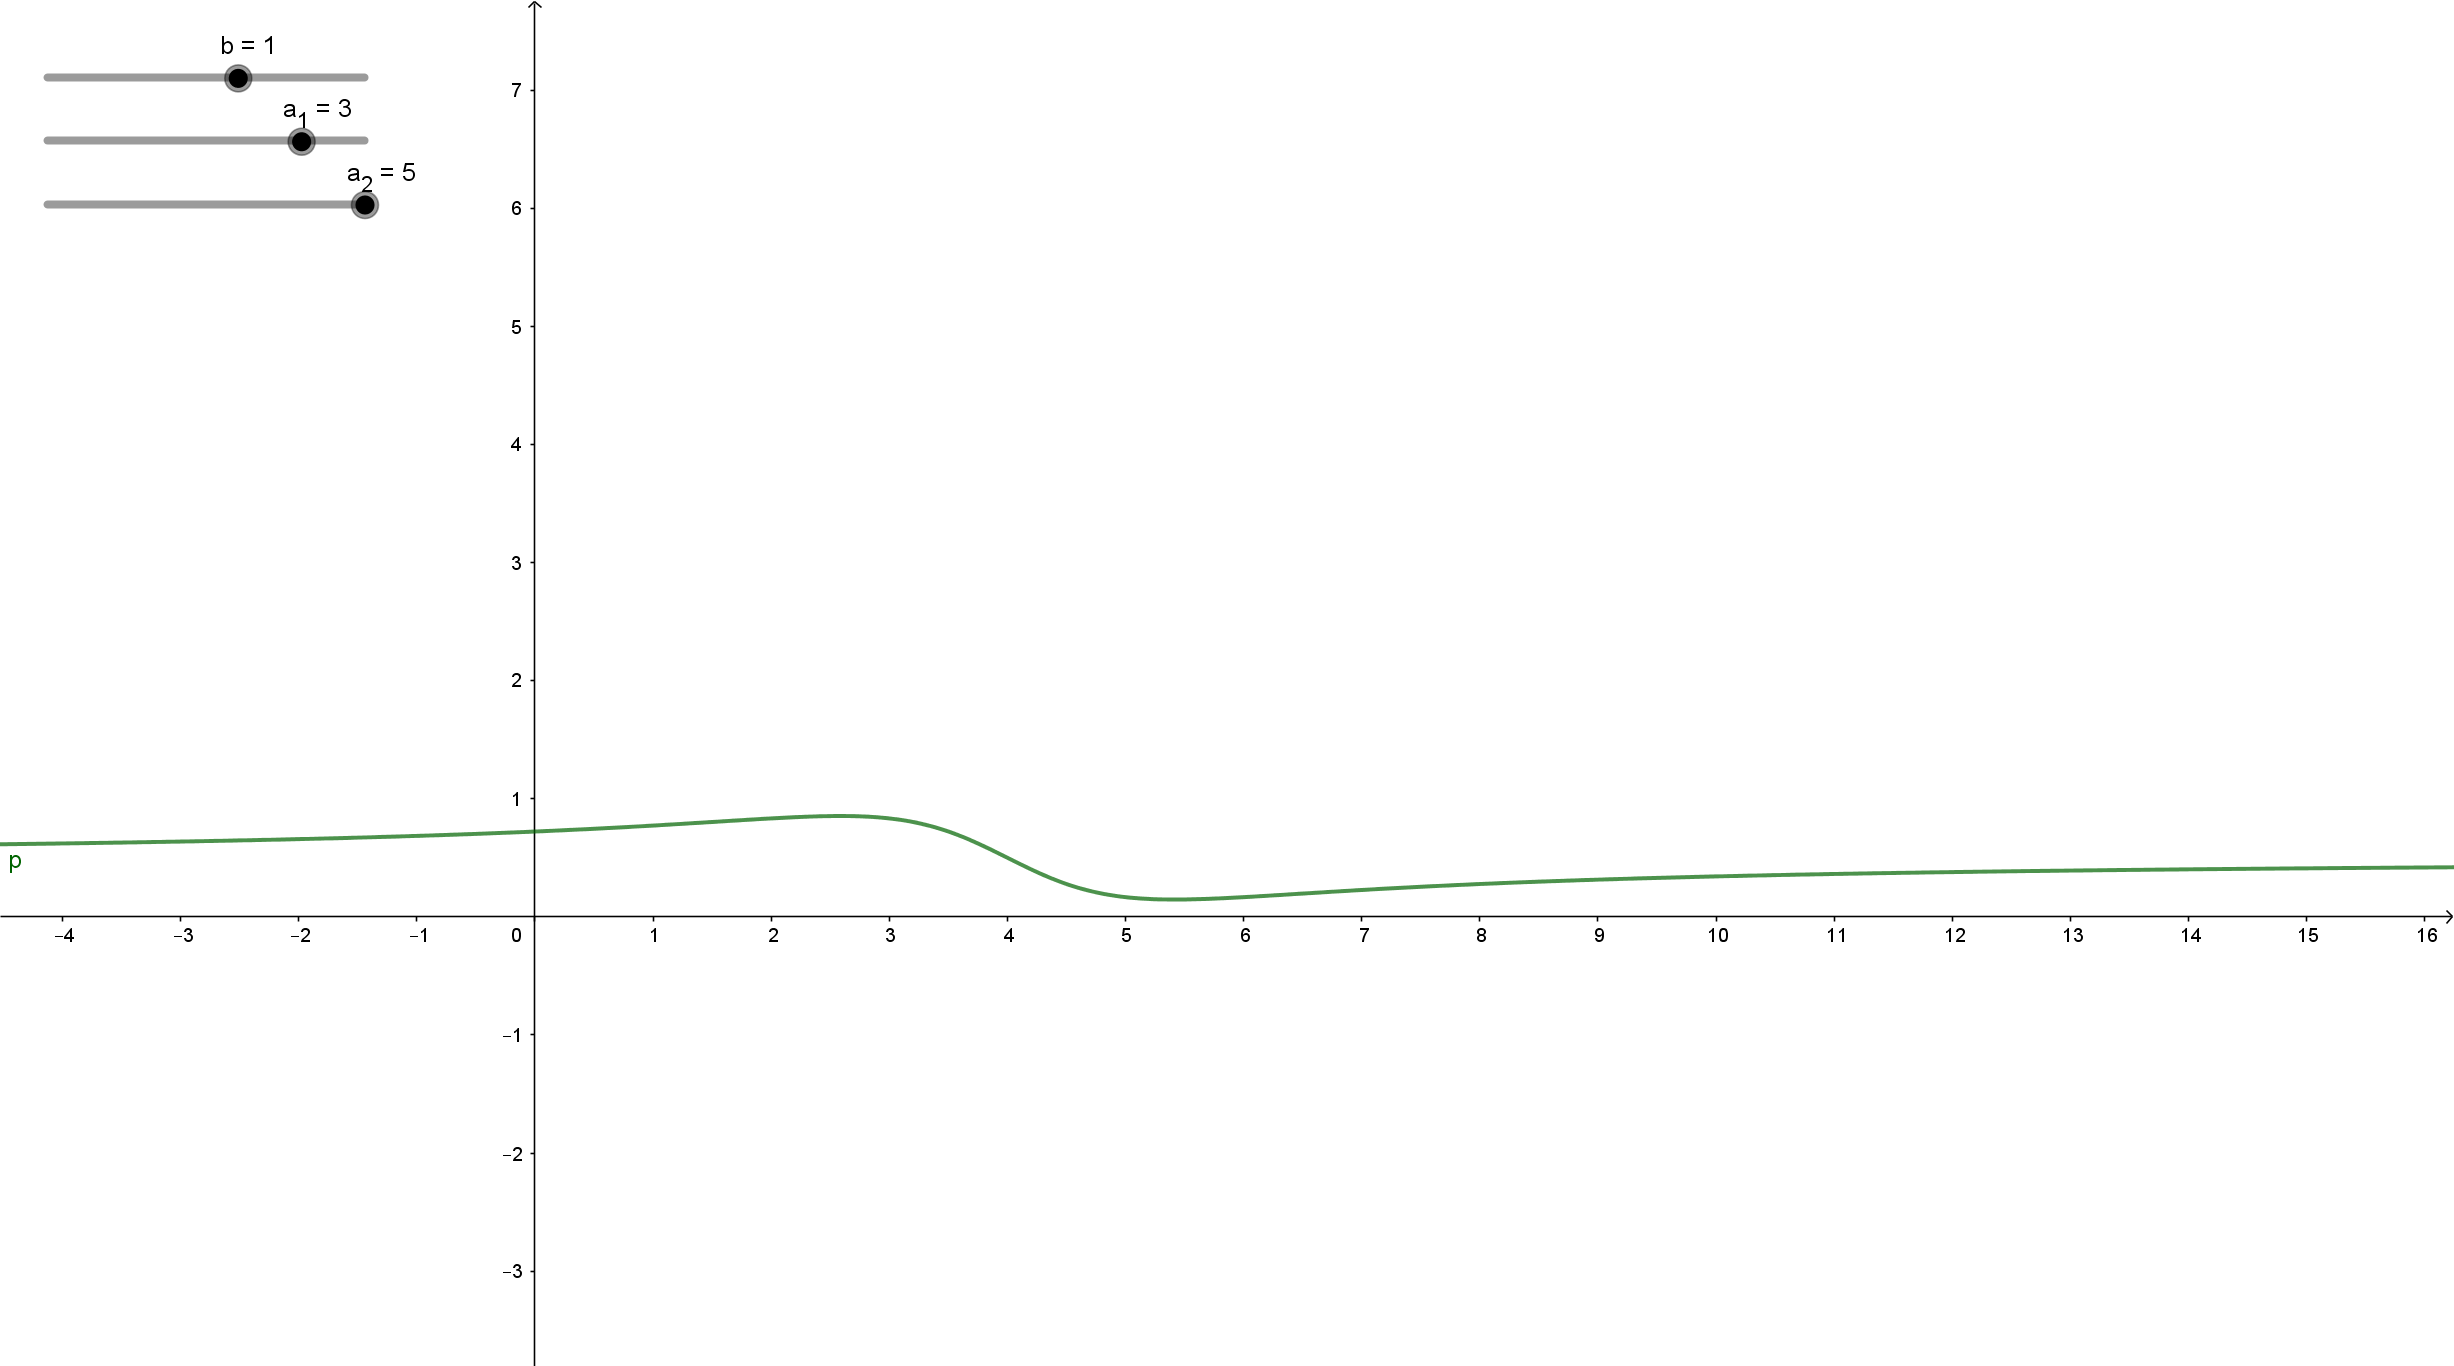
\includegraphics[scale=0.4]{7c}
\end{figure}
The function increases until 3, where has a maximum, decreases until 5, where have a minimum, and increases again. It also has two asymptotes as we will see in the section (d). \\ 
\Large
  \item[(d)] How do $P(w_1|x)$ and $P(w_2|x)$ behave as $x \rightarrow -\infty$? $x \rightarrow +\infty$? Explain.\\ \ \\
\normalsize
As we can see in the plot, in $P(w_1|x)$, when $x \rightarrow -\infty$, the function tends to 0.5 from above, so 0.5 is an asymptote. Similarly when $x \rightarrow +\infty$ the distribution tends to 0.5, but now from below. Again, 0.5 is an asymptote. \\ 

As $P(w_2|x)=1-P(w_1|x)$, the behavior of $P(w_2|x)$ is the opposite of $P(w_1|x)$. When $x \rightarrow -\infty$, $P(w_2|x)\rightarrow 0.5$ from below and when $x \rightarrow +\infty$, $P(w_2|x)\rightarrow 0.5$ from above. So similarly, the function has two asymptotes at 0.5. \\

We can show it analytically. First, notice that $P(w_1|x)$ (as a function of $x$) can be simplified and written as:
$$
P(w_1|x) = \frac{x^2 - 10x + 26}{2x^2-16x+36}
$$ 
From where the asymptotes when $x \rightarrow \pm\infty$ can be easily seen that are a half. Because it is a fraction of polynomials, and the asymptote is the fraction of the coefficients of the components with 2 in the exponent. Now, to see if it is from below or above or none of them we have to check the following inequality:
$$
P(w_1|x) =\frac{x^2 - 10x + 26}{2x^2-16x+36}>0.5
$$
As the denominator is positive always, the inquality is equivalent to:
$$
x^2 - 10x + 26 > x^2-8x+18
$$
So, simplifying, the inequality occurs when:
$$
x < 4
$$
And, if we want to see when $P(w_1|x) < 0.5$ the operations are the same, and results $ x > 4$. Therefore, when $x \rightarrow -\infty$, 
$P(w_1|x)\rightarrow 0.5$ from above, and when $x \rightarrow +\infty$, $P(w_1|x) \rightarrow 0.5$ from bellow. As it has been explain before, this behavior inverts in $P(w_2|x)$ so no more computation is needed.


\end{enumerate}



\end{document} 